\chapter{Einleitung}
Das Thema \ac{KI} erlangt zunehmend an Relevanz und durchdringt viele Felder. Auch die Hochschullehre kann vom Einsatz künstlicher Intelligenzen profitieren. Es existieren erste Versuche intelligente Systeme in die Lehre zu integrieren, wie etwa Chatbots in eingesetzten Lernmanagementsystemen, qualitative Auswertungen von Lernendendaten durch Learning Analytics und weitere \cite*[S. 18, S. 14ff.]{Witt.2020}.

Abbilung \ref*{fig:entwickling_ki} veranschaulicht die Entwicklung der Verbreitung von \ac{KI} generell und in der Kategorie \glqq Studium und Lehre\grqq. Es ist eine Tendenz dahin erkennbar, dass generell künstliche Intelligenz zunehmend vorkommt. Zudem ist KI in der Rubrik Studium und Lehre zwar relativ seltener vertreten, aber die Tendenz steigt.
\begin{figure}[hbtp]
    \centering
    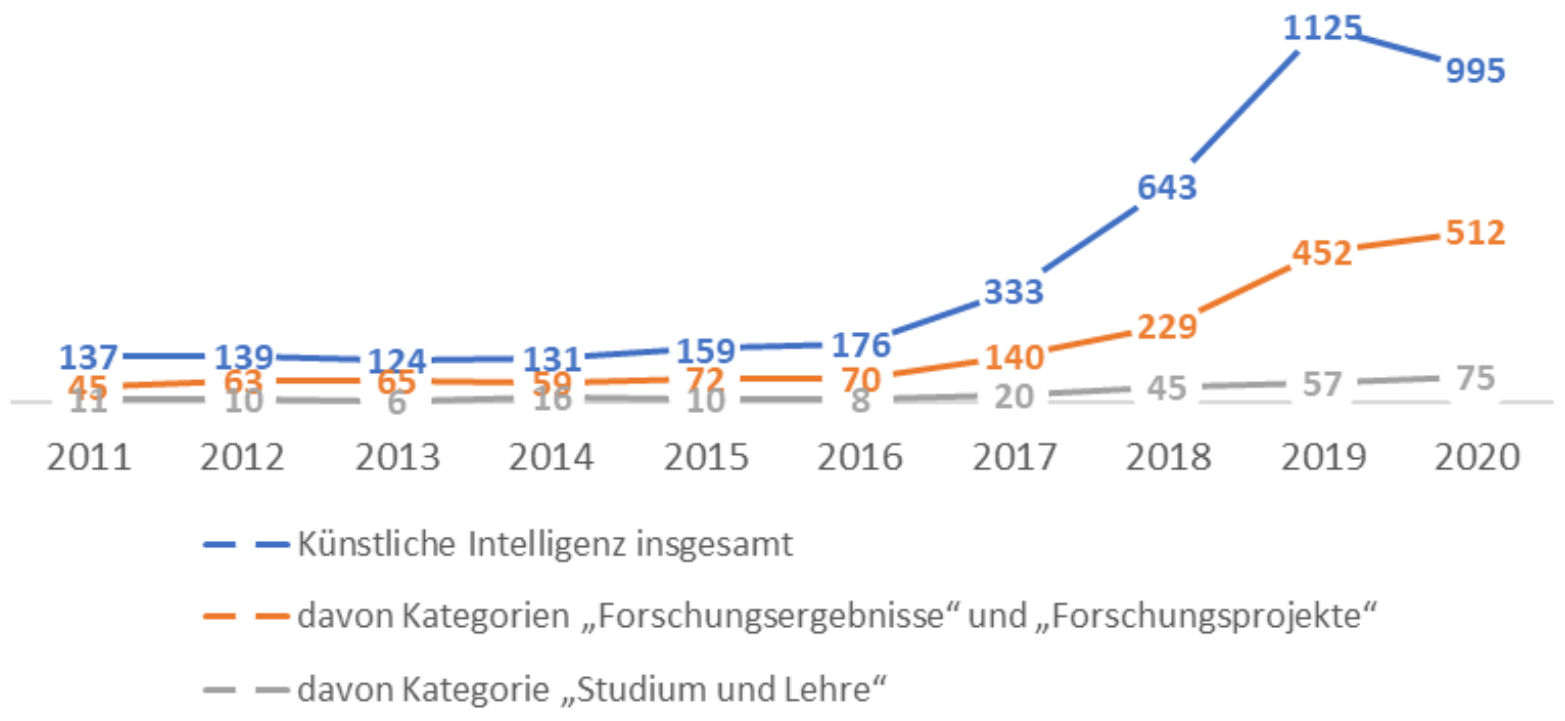
\includegraphics[width=.8\textwidth]{figures/entwicklung_historie_ki.png}
    \caption{Anzahl der Pressemitteilungen von Hochschulen und weiteren Wissenschafts-Institutionen, die das Schlagwort „Künstliche Intelligenz“ enthalten \cite*[S. 9]{Wannemacher.2021}}
    \label{fig:entwickling_ki}
\end{figure}

Zugriffsdaten sind Daten, die beim Zugriff auf (Web-)Ressourcen erzeugt werden. Sie können bspw. für das Reporoduzieren und Beheben von Fehlern eingesetzt werden. Daher ist davon auszugehen, dass sie in Systemen in großen Mengen vorhanden sind. Sie können jedoch auch für Analysezwecke genutzt werden, um vom Zugriffsverhalten Rückschlüsse auf andere Erkenntnisse zu erlangen.

Für die Entwicklung von KIs sind Daten notwendig, welche für das Training einer der KI eingesetzt werden. Hochschulen setzen in großen Teilen bereits Systeme für die Lehre ein und besitzen demnach Daten, besonders Zugriffsdaten. Die zentrale Arbeitsfrage dieser Ausarbeitung ist, wie Zugriffsdaten für den Einsatz von künstlichen Intelligenzen im Kontext der Hochschullehre eingesetzt werden können.

Hierfür wird zunächst eine Einführung in das Themenfeld KI im Kontext der Hochschullehre gegeben. Die Paper \glqq Künstliche Intelligenz in der Hochschullehre\grqq{} von de Witt, Rampelt und Pinkwart und \glqq Another 25 Years of AIED? Challenges and Opportunities for Intelligent Educational Technologies of the Future\grqq{} von Pinkwart geben einen Überblick über aktuelle Entwicklungen in der Hochschullehre mit KIs. Hierfür werden die Erkenntnisse der Paper herausgestellt. Anschließend folgt eine Analyse einer KI, die im \ac{LMS} Moodle die Zugriffsdaten des \ac{LMS} auswertet. Die Ergebnisse werden im Fazit zusammengefasst und eine Bewertung zu den Entwicklungen gegeben.